\documentclass[9pt,twocolumn,twoside]{revtex4-1}

\usepackage{graphicx}
\usepackage{dcolumn}
\usepackage{bm}
\usepackage{natbib}
\usepackage{physics}

\newcommand{\bea}{\begin{eqnarray}}
\newcommand{\eea}{\end{eqnarray}}

\begin{document}
\title{Optical Detection of Paramagnetic Defects in a CVD-grown diamond\\-- Supplementary Material}

\author{C. Pellet-Mary$^{1}$}
\author{P. Huillery $^{1}$}
\author{M. Perdriat $^{1}$}
\author{A. Tallaire $^{2}$}
\author{G. H\'etet$^{1}$} 

\affiliation{$^1$Laboratoire de Physique de l'Ecole normale sup\'erieure, ENS, Universit\'e PSL, CNRS, Sorbonne Universit\'e, Universit\'e Paris-Diderot, Sorbonne Paris Cit\'e, Paris, France.}
\affiliation{$^2$IRCP, Ecole Nationale Supérieure de Chimie de Paris, 11, rue Pierre et Marie Curie, 75005 Paris, France}


\maketitle

\section{Photoluminescence as a function of the magnetic field for a HPHT sample}

The NV$^-$ photoluminescence as a function of the magnetic field amplitude that is presented in the Fig. 3 of the main text was realized on a CVD-grown sample. 
We also performed similar scans on several samples grown via the High-Pressure-High-Temperature (HPHT) method. 
Fig. \ref{fig1SI} shows a scan realized on HPHT samples that have been irradiated in order to increase the NV yield. 
The sample we use in Fig. \ref{fig1SI} is a Ib electron irradiated HPHT diamond crystal with a NV concentration expected to be in the 5-20 ppm range.
The PL feature that can be observed at 20G was also observed in the CVD-grown samples. We attributed it to the resonant dipolar interaction between a standard polarized NV center and one NV strongly coupled to the nuclear spin of a $^{13}$C atom sitting one shell away.
Notably, no other features could be detected at larger magnetic field values. We realized such scans on many different highly-doped HPHT samples and, systematically, no CR features are observed at 50 and 122 G. 

 \begin{figure}[htbp]
\centering
{\includegraphics[width=\linewidth]{sumi4_13C.eps}}
\caption{NV$^-$ photoluminescence rate while scanning the magnetic field along the [100] crystalline direction. Here a HPHT sample was employed.}
\label{fig1SI}
\end{figure}

\section{NV-$^{13}$C Hamiltonian}

The full spin Hamiltonian of the NV-$^{13}$C complex can be written as follows : 
\begin{equation*}
\mathcal{H}=\mathcal{H}_{NV}+\mathcal{H}_{^{13}C}+\mathcal{H}_{HF},
\end{equation*}
where $\mathcal{H}_{NV}$ is the NV$^-$ spin Hamiltonian.
For one NV orientation, with quantization axis $z$, it reads 
\begin{equation}\hat{H}_{\rm NV}=\hbar D \hat{S}_z^2+ \hbar \gamma_e \bf B  \cdot \bf\hat S.
\end{equation}
$D$ is the zero-field-splitting and $\bf\hat S$ is the electronic spin operator.
$\mathcal{H}_{^{13}C}$ is the $^{13}$C nuclear spin Hamiltonian for a $1/2$ spin : $\mathcal{H}_{^{13}C}=\gamma_{n} B I_z$ where $\gamma_{n}=$10.7 MHz/T is the $^{13}$C gyromagnetic ratio, and $\mathcal{H}_{HF}$ is the hyper-fine interaction Hamiltonian : $\mathcal{H}_{HF}= \hat{\mathbf{S}}_{NV} \cdot \mathcal{A} \cdot \hat{\mathbf{I}}_C$.

In the case of a first shell $^{13}$C, the hyper-fine tensor $\mathcal{A}$ can be written as \citep{simanovskaia_sidebands_2013} : $$ \mathcal{A} = \begin{pmatrix}
\mathcal{A}_{xx} & 0 & \mathcal{A}_{xz} \\ 0 & \mathcal{A}_{yy} & 0 \\ \mathcal{A}_{zx} & 0 & \mathcal{A}_{zz}
\end{pmatrix},$$
where $\mathcal{A}_{xx}=190.2(2)$ MHz, $\mathcal{A}_{yy}=120.3(2)$ MHz, $\mathcal{A}_{zz}=129.1(2)$ MHz, and  $\mathcal{A}_{xz}=\mathcal{A}_{zx}=-25.0(1)$ MHz. 

Diagonalizing the total Hamiltonian, we notice that the quantization axis of the nuclear spin (in the limit $\gamma_{n} B \ll A_{ij}$) is not the same in the manifold of the $\ket{m_s=0}$ state and in the $\ket{m_s=\pm 1}$ states \citep{alvarez_local_2015}, meaning that the nuclear spin is not preserved by the electron spin flip, and gives rise to a splitting of the $\ket{m_s=0} \to \ket{m_s=\pm 1}$ transition in 4 distinct lines when the magnetic field is not aligned with the NV center \citep{jiang2018estimation}.

\section{NV-P1 mutual spin flip transitions}

Transitions corresponding to a simultaneous flip of the NV$^-$ and P1 (substitutional nitrogen) spin states, mediated by the dipolar interaction between NV$^-$ and P1 electronic spins, are commonly observed on ODMR spectra \citep{simanovskaia_sidebands_2013, kamp2018continuous, alfasi2019detection, lazda2020cross}. Here, we investigate whether the cross-relaxation processes we observe could be partly due a three-body interaction between two NV centers and one P1 center.

In order for this process to be energy conserving, the P1 transition frequency has to match the energy difference between the $\ket{m_s=0} \to \ket{m_s=-1}$ and $\ket{m_s=0} \to \ket{m_s=+1}$ transitions, giving us the equation \begin{equation}
\label{eq_P1}
\nu^i_{P1}(B)=\nu^{0 \to +1}_{NV}(B)-\nu^{0 \to +1}_{NV}(B),
\end{equation}
where $\nu^i_{P1}$ is a transition between any of the P1 spin Hamiltonian eigenstates. Note that since we are scanning the magnetic field in the crystalline [100] direction, we do not have to take into account the four classes of NV centers and P1.

The P1 spin states are defined by its electron 1/2-spin and its nuclear 1-spin, giving a manifold of 6 spin states. When considering any possible transitions between the 6 eigenstates of the P1 Hamiltonian, we have therefore a total of 15 possible transitions, including the nuclear-like transitions which have been observed through mutual spin flip with NV centers \citep{alfasi2019detection}. 

%Solving eq. \ref{eq_P1} for all possible P1 transitions (see fig. \ref{fig_P1}) therefore gives us all the possible magnetic field amplitude in the [100] direction where we could observe NV-P1 mutual flip transitions. The predicted magnetic field values are 0, 3.89, 5.96, 6.58, 17.90, 28.93, 35.87, 49.44, 81.33, 83.28, 137.52, 154.20 and 246.34 G. None of these values correspond to one of the feature our scans. We then concluded that the Features we observed were not due to NV-P1 mutual flips. 

Using the numerical values of the P1 Hamiltonian from \citep{lazda2020cross}, we solve Eq. \ref{eq_P1} for all possible P1 transitions (see fig. \ref{fig_P1}) therefore giving us all the possible magnetic field amplitudes in the [100] direction where we could observe NV-P1 mutual spin flip transitions. The predicted magnetic field values are 0, 3.89, 5.96, 6.58, 17.90, 28.93, 35.87, 49.44, 81.33, 83.28, 137.52, 154.20 and 246.34 G. None of these values correspond to any feature in our scans. We then concluded that the features we observed were not due to NV-P1 mutual flips.

\begin{figure}
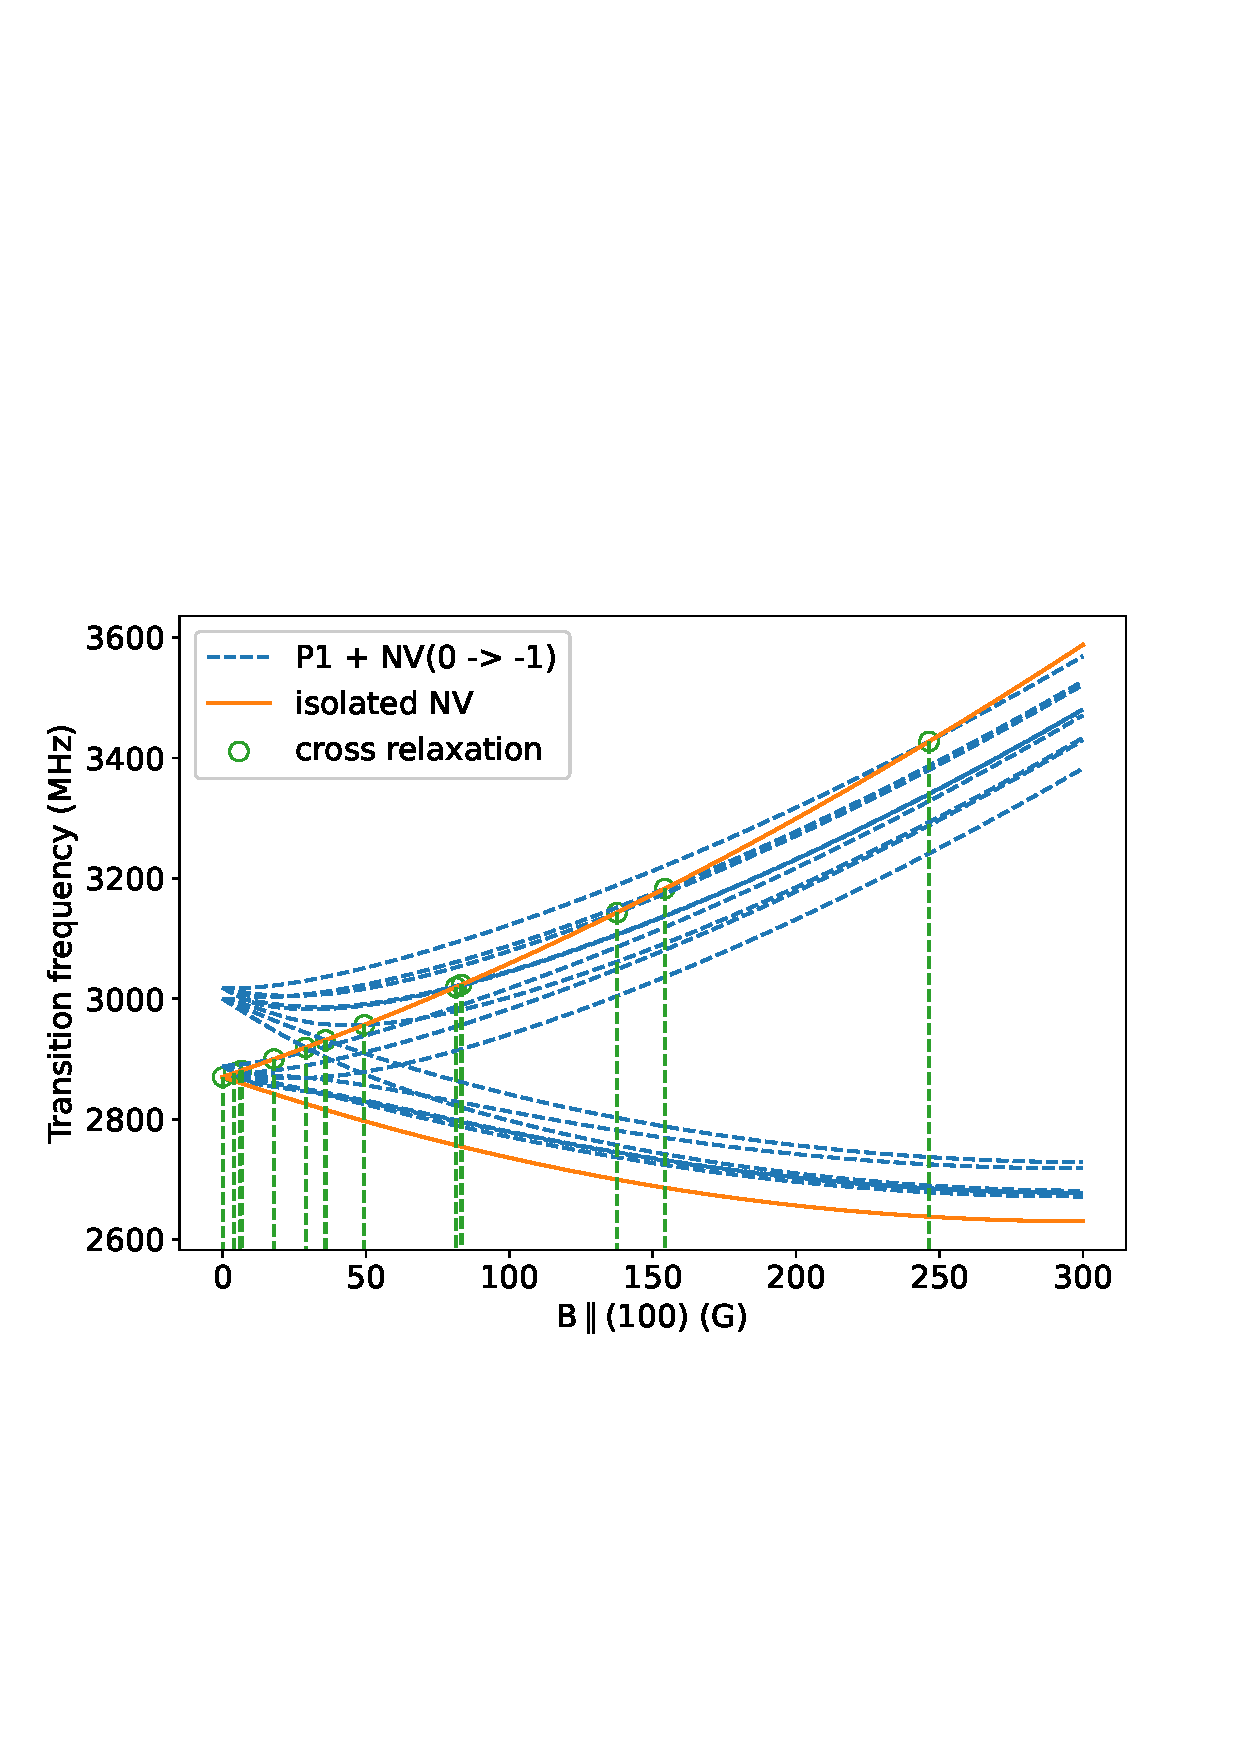
\includegraphics[width=\linewidth]{Transis_P1}
\caption{Cross-relaxation condition for mutual flip between NV and P1 centers. The orange plain lines correspond to the NV center $\ket{m_s=0} \to \ket{m_s=-1}$ and $\ket{m_s=0} \to \ket{m_s=+1}$ transition frequencies as function of a magnetic field along the [100] crystalline axis, the blue dashed lines correspond to the frequencies of the 15 theoretical transitions of the P1 centers, added to the frequency of the NV $\ket{m_s=0} \to \ket{m_s=-1}$ transition. The green circles correspond to the particular magnetic fields where Eq. \ref{eq_P1} is verified, meaning where the energy of the P1 transition matches the energy difference between the two NV transitions.}\label{fig_P1}
\end{figure}
% Bibliography
\bibliographystyle{plain}

\section{Scan in the [111] direction}
\begin{figure}
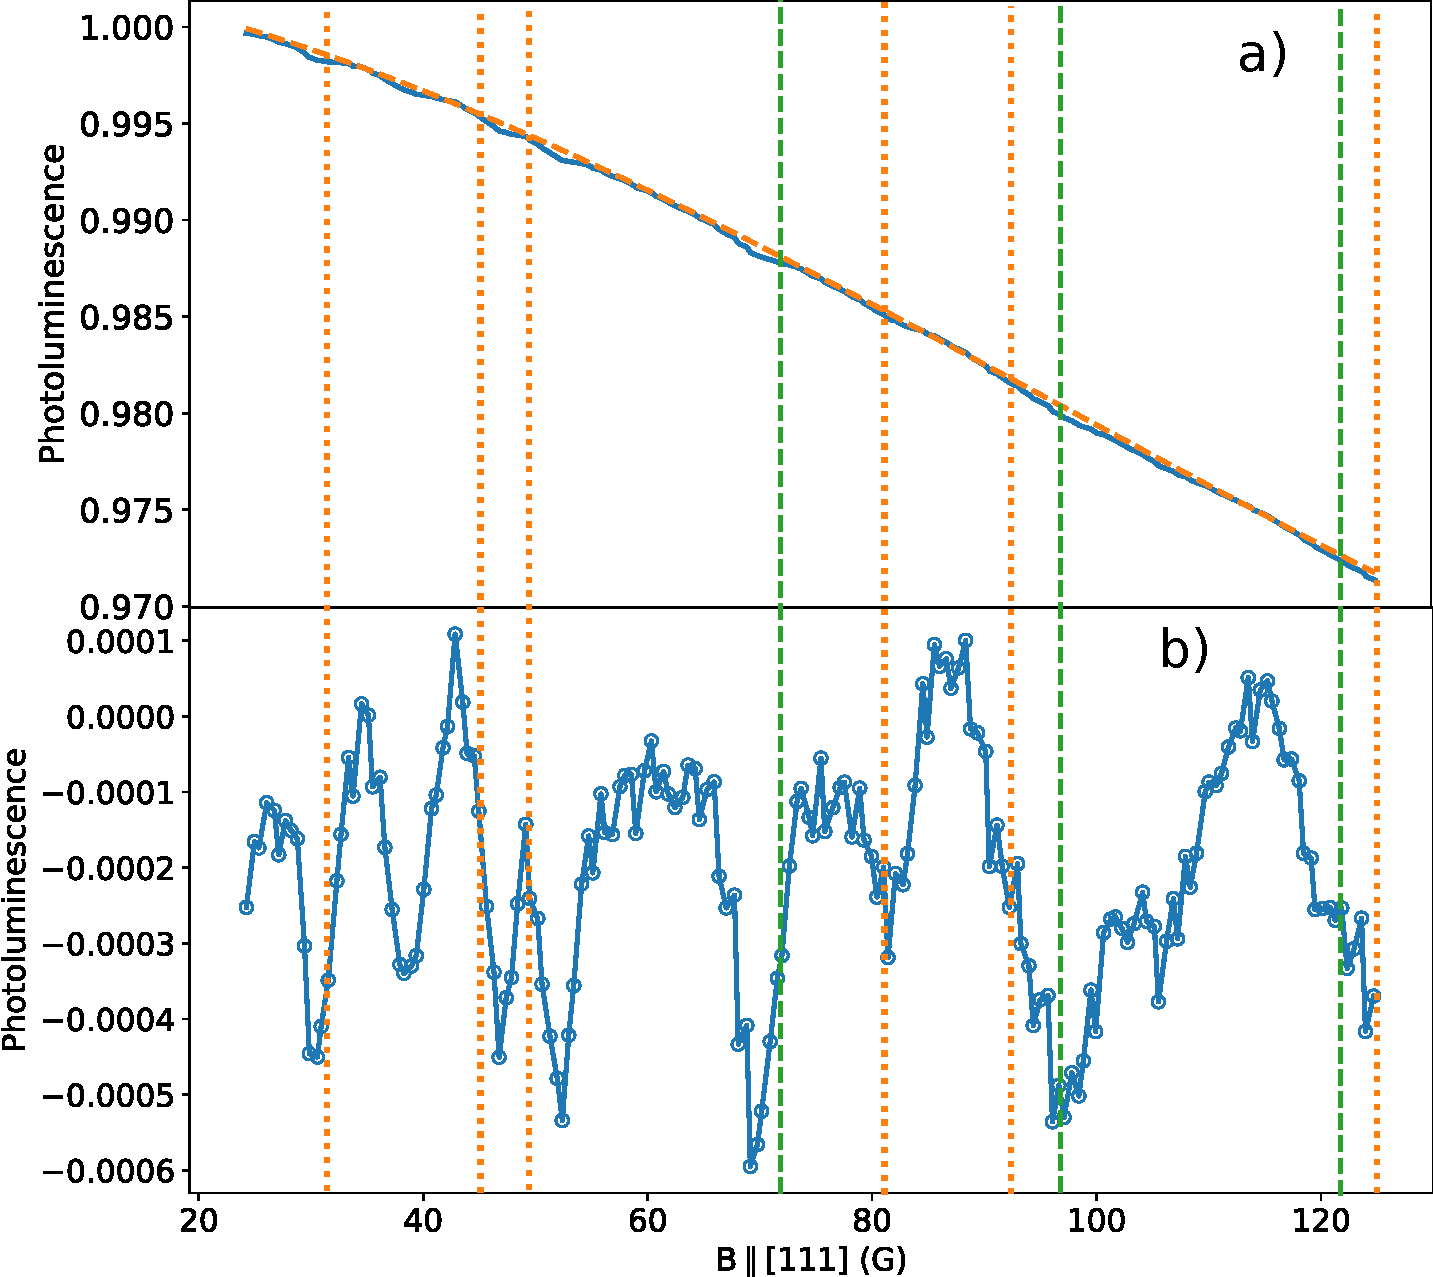
\includegraphics[width=\linewidth]{scan_111_PL}
\caption{\textbf{a)} Plain blue line : Photoluminescence as a function of the magnetic field amplitude in the [111] crystalline direction. Dashed orange line : 4th order polynomial fit of the decreasing envelope. \textbf{b)} Subtraction of the previous signal by the envelope fit. The vertical dotted orange lines correspond to the expected cross-relaxations with VH$^-$ and the vertical dashed green lines to the expected cross-relaxations with WAR1.}\label{scan_PL}
\end{figure}

\begin{figure}
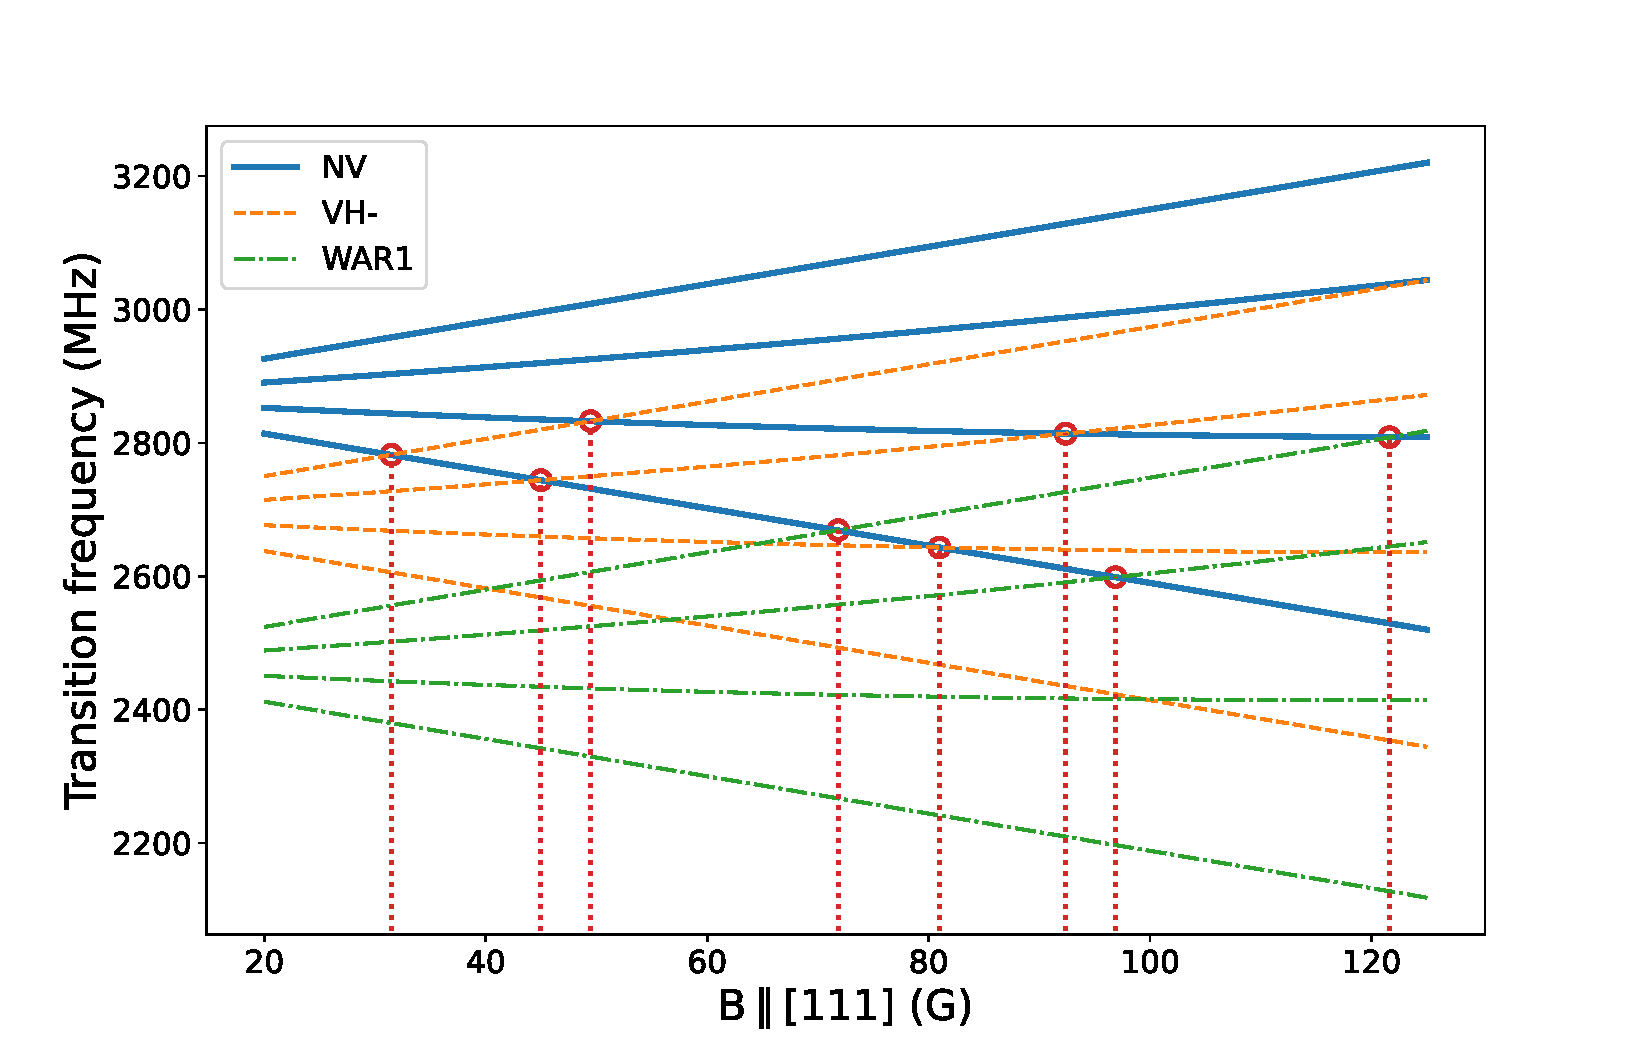
\includegraphics[width=\linewidth]{Transis_111_VHWAR}
\caption{Predicted transition frequencies of NV$^-$ centers (plain lines), VH$^-$ (dashed lines) and WAR1 (dash-dotted lines) when the magnetic field is scanned in the [111] direction. The magnetic field values for which  a transition of the NV center crosses one of VH$^-$ or WAR1 are also shown in Fig \ref{scan_PL}.}\label{transis_VHWAR}
\end{figure}

\begin{figure}

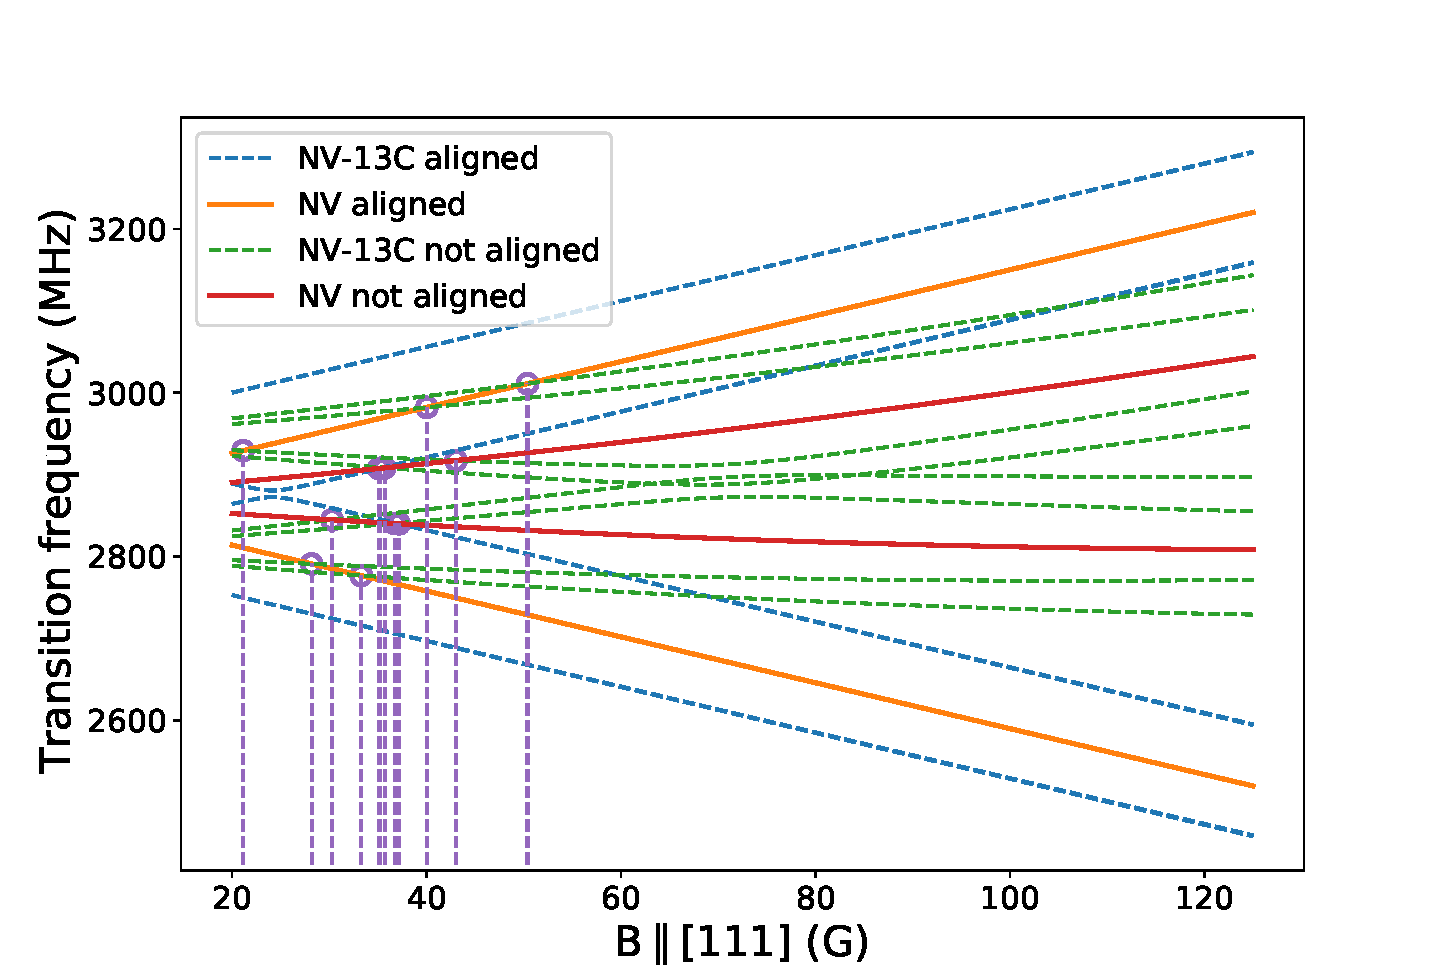
\includegraphics[width=\linewidth]{Transis_111_13C}
\caption{Predicted transitions frequencies for NV centers (plain lines) and NV-$^{13}$C complex when the magnetic field is scanned in the [111] direction. Vertical lines represent the various degeneracy conditions.}\label{transis_13C}
\end{figure}

We have performed similar magnetic field scan as presented in Fig.3 of the main text, but scanning the magnetic field in the crystalline [111] direction instead of the [100], meaning that this time one class of NV centers is aligned with the magnetic field while the three others are misaligned and degenerate. The results in term of cross-relaxations generally means 4 times as many degeneracy conditions as the [100] case, since the two spins involved in the cross-relaxation process now have two possible orientations, and therefore two separate transitions.

It is then significantly harder to find cross-relaxations signatures, since they are both more numerous and with a smaller contrast than in the [100] case. The experimental results are shown in Fig. \ref{scan_PL}. Similarly to Fig. 3 of the main text, we have subtracted the envelope associated with the transverse field in order to better see the fine features of the scan. The predicted cross-relaxation conditions between NV centers and VH$^-$ or WAR1 are presented in fig. \ref{transis_VHWAR} and shown in Fig. \ref{scan_PL}. While the predicted values do not exactly match the experimental results, it seems like every predicted transition falls in the vicinity of an experimental line. Importantly, it should be noted that, unlike Fig.3 of the main text, the magnetic field was not calibrated with the lengthy NV ODMR at every field value in this case. Instead we have simply applied a homotethy on the current intensity in the electromagnet to match the field values at the maxima of the scan. This means that the magnetic field of the points of low field value in particular are more susceptible to the non-linearities due to the electromagnet hysteresis cycle.

Finally we have plotted in Fig.\ref{transis_13C} the expected cross-relaxations between NV and NV-$^{13}$C complex. It seems that these transitions are too diluted to appear in our experimental scan. The peak at $\sim$37 G in fig.\ref{scan_PL} could come from the resonance between NV and NV-$^{13}$C since they seem particularly dense at this particular field values.
It is indeed  the only peak that is not matching any of the NV-VH$^-$ or NV-WAR1 resonance.

\section{Fitting of the cross-relaxation scans}
\begin{figure}
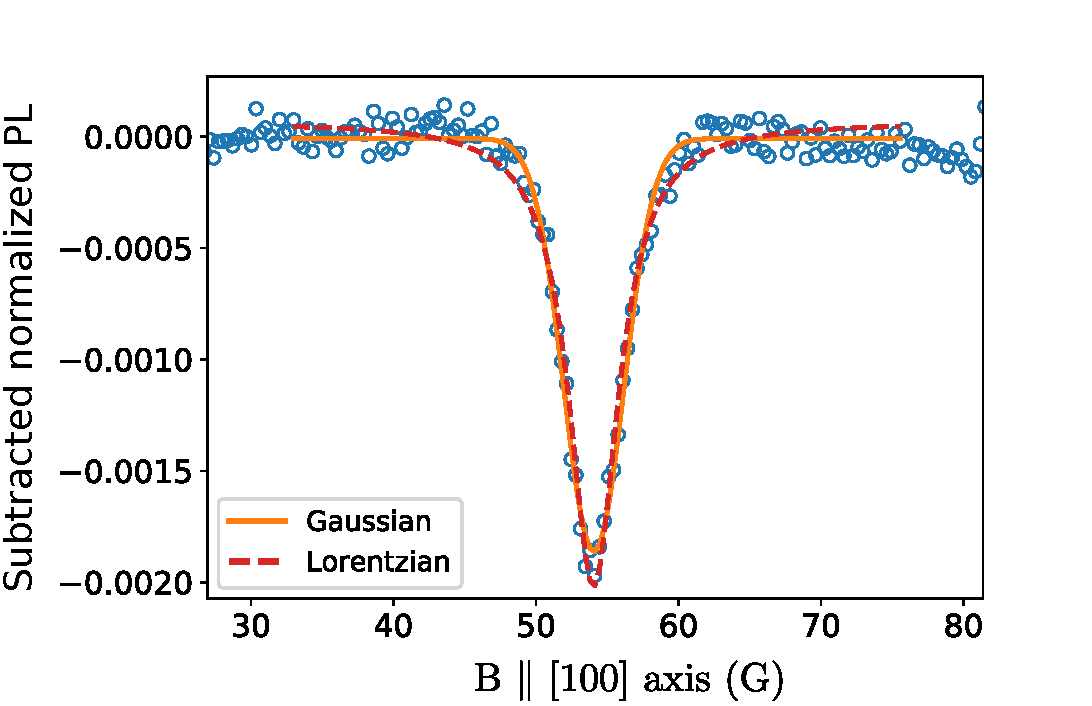
\includegraphics[scale=0.5]{Gauss_vs_Lor_VH}
\caption{Zoom-in on the VH$^-$ cross-relaxation line from Fig.3 of the main text with Gaussian (orange,plain line) and Lorentzian (red, dashed line) fit}
\label{Gauss_vs_Lor}
\end{figure}
In order to extract quantitative information from Fig.3 of the main text, we had ta apply two distinct fits to the raw data : first a polynomial fit to subtract the slowly decaying PL due to sate-mixing, then a Lorentzian fit on the VH$^-$ and WAR1 resonance lines to measure the central position, width and amplitude of the lines.

For the subtracting fit, we chose a polynomial fit because numerical solving of the transverse-field dependent spin depolarization could not properly fit our results. We had to use up a 4th order polynomial in order to obtain a tight fit to the data. Higher order polynomials did not significantly change the fitting envelope.

The second and third peaks were fitted better on their wings by a Gaussian than by a Lorentzian lineshape, as can be seen in Fig. \ref{Gauss_vs_Lor} where the Gaussian fit yields a $R^2=0.983$ greater than the $R^2=0.974$ from the Lorentzian fit. This is coherent with the fact that the inhomogeneous broadening of the various spin species dominates the coupling strength between the spins.

\section{Sample fabrication details}
The main CVD sample of this study is presented in thorough details in \citep{TALLAIRE2020421}. It is a thick (100) oriented diamond grown in-house by CVD with an initial concentration [N]$\approx$25~ppm and separated from its HPHT substrate. It was electron irradiated at 10MeV and a fluence of $2\cdot 10^{18}$~cm$^{-2}$ and in situ annealed at 900°C during irradiation to give a final concentration [NV]$\approx$4.6~ppm.

The HPHT sample used in Sec.I of the supplementary material is a thick (111)-oriented diamond from Sumitomo and was electron irradiated at an energy of 2 MeV and a fluence of $7\cdot 10^{18}$~cm$^{-2}$. It was then annealed in vacuum for 2h at 950°C.

We also tried the same experiment on similar HPHT samples with a fluence ranging from $4\cdot 10^{18}$~cm$^{-2}$ to $1.5\cdot 10^{18}$~cm$^{-2}$, as well as on several heavily doped 15 $\mu$m diamonds bought from Adamas Nanotechnologies, and all the HPHT sample showed a feature at $\sim$20~G, but none of them showed any feature at 56 or 125~G.

\begin{thebibliography}{1}

\bibitem{alfasi2019detection}
Nir Alfasi, Sergei Masis, Oleg Shtempluck, and Eyal Buks.
\newblock Detection of paramagnetic defects in diamond using off-resonance
  excitation of nv centers.
\newblock {\em Physical Review B}, 99(21):214111, 2019.

\bibitem{jiang2018estimation}
Feng-Jian Jiang, Jian-Feng Ye, Zheng Jiao, Zhi-Yong Huang, and Hai-Jiang Lv.
\newblock Estimation of vector static magnetic field by a nitrogen-vacancy
  center with a single first-shell 13c nuclear (nv--13c) spin in diamond.
\newblock {\em Chinese Physics B}, 27(5):057601, 2018.

\bibitem{kamp2018continuous}
EJ~Kamp, B~Carvajal, and N~Samarth.
\newblock Continuous wave protocol for simultaneous polarization and optical
  detection of p1-center electron spin resonance.
\newblock {\em Physical Review B}, 97(4):045204, 2018.

\bibitem{lazda2020cross}
Reinis Lazda, Laima Busaite, Andris Berzins, Janis Smits, Marcis Auzinsh,
  Dmitry Budker, Ruvin Ferber, and Florian Gahbauer.
\newblock Cross-relaxation studies with optically detected magnetic resonances
  in nitrogen-vacancy centers in diamond in an external magnetic field.
\newblock {\em arXiv preprint arXiv:2007.00473}, 2020.

\bibitem{simanovskaia_sidebands_2013}
Maria Simanovskaia, Kasper Jensen, Andrey Jarmola, Kurt Aulenbacher, Neil
  Manson, and Dmitry Budker.
\newblock Sidebands in optically detected magnetic resonance signals of
  nitrogen vacancy centers in diamond.
\newblock {\em Phys. Rev. B}, 87(22):224106, June 2013.

\bibitem{TALLAIRE2020421}
Alexandre Tallaire, Ovidiu Brinza, Paul Huillery, Tom Delord, Clément
  Pellet-Mary, Robert Staacke, Bernd Abel, Sébastien Pezzagna, Jan Meijer,
  Nadia Touati, Laurent Binet, Alban Ferrier, Philippe Goldner, Gabriel Hetet,
  and Jocelyn Achard.
\newblock High nv density in a pink cvd diamond grown with n2o addition.
\newblock {\em Carbon}, 170:421 -- 429, 2020.

\bibitem{alvarez_local_2015}
Gonzalo~A. Álvarez, Christian~O. Bretschneider, Ran Fischer, Paz London, Hisao
  Kanda, Shinobu Onoda, Junichi Isoya, David Gershoni, and Lucio Frydman.
\newblock Local and bulk {13C} hyperpolarization in nitrogen-vacancy-centred
  diamonds at variable fields and orientations.
\newblock {\em Nat Commun}, 6(1):8456, December 2015.

\end{thebibliography}


\end{document}
